%!TEX root = ../thesis.tex
%*******************************************************************************
%****************************** Second Chapter *********************************
%*******************************************************************************

\chapter{Simple 1-Dimentional Problem}

\ifpdf
    \graphicspath{{Chapter2/Figs/Raster/}{Chapter2/Figs/PDF/}{Chapter2/Figs/}}
\else
    \graphicspath{{Chapter2/Figs/Vector/}{Chapter2/Figs/}}
\fi


\section[Short title]{Illustration of Basic Principles}

% Uncomment this line, when you have siunitx package loaded.
By constraining $\bm{x}$ to one dimention allows for the problem to be simplified. Suppose ${f(x)=\sin(x)+0.05x^2}$ with ${x\in [-10, 10]}$ as shown in Figure~\ref{fig:firstFunction}. In this range, there are multiple minima with only one global minima. The task here is to successfully locate the minima situated at -1.428 (found through ananlytical differentiation and solving ${10\cos(x)+x=0}$). This will be compared against two benchmarks: linear spacing and the fminbound method available in the scipy package given the same number of function calls. $\epsilon$ will be chosen to be independent of $x$ and $y$ and fit a normal distribution such that $\epsilon\sim N(0, 1)$.

\begin{figure}[htbp!] 
\centering    
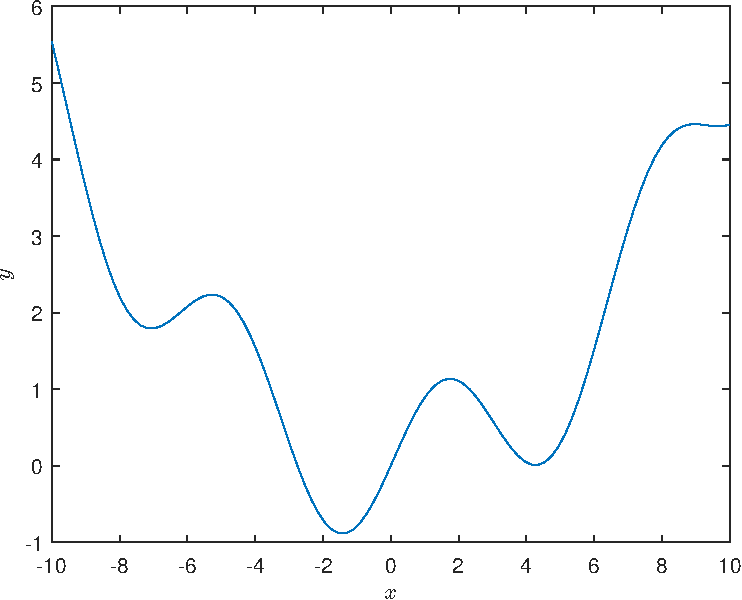
\includegraphics[width=1.0\textwidth]{firstFunction.pdf}
\caption[First Function]{$y = \sin(x) + 0.005x^2$ with $x\in [-10, 10]$}
\label{fig:firstFunction}
\end{figure}



\subsubsection{Linear Selection}
The least inteligent method while not being deliberately obtuse is linearly spacing sampled values and choosing $x$ equal to the lowest sampled value. This does have the advantage that all experimentations may be construed asynchronously. Thus, where material and labour cost is low, this may be beneficial.
\subsubsection{Active Learning}
This methodolgy has two underlying core principles: sparse areas reveal the most information and minimal areas reveal information to the location of the minima. Combining these allows for better decision making with regards to the next sample to choose.

There are several methods that may be used to enhance this strategy. Firstly, a smoothing spline between points allows for a non-parametric fit of the data to be used. Alternatively, a local regression fit may be used allowing for changes in sample density. Advanced methods using Baysian Statistics and advanced information theory may be used, although have been ommitted due to time restraints.

In this paper, three functions are found: $e(x)$, $p(x)$ and $h(x)$, denoting a guessed fit, the sparcity, and the height respectively. $p(x)$ is defined between adjacent samples, $s_i$.
\begin{equation}
  {h(x)=-e(x)+\max[e(x)]}
\end{equation}
\begin{equation}
  p(s_i \le x \le s_{i+1})=-\left|x-\frac{s_i+s_{i+1}}{2}\right|+\frac{s_{i+1}-s_{i}}{2}
\end{equation}
\begin{equation}
  p(s_i \le x \le s_{i+1})=\min[x-s_i, s_{i+1}-x]
\end{equation}
\subsubsection{fminbound}
fminbound is a function included in the scipy optimisation library. It uses Brent's method allowing it to be quick in situations where labeling is quick and error is low.

\begin{enumerate}
\item The first topic is dull
\item The second topic is duller
\begin{enumerate}
\item The first subtopic is silly
\item The second subtopic is stupid
\end{enumerate}
\item The third topic is the dullest
\end{enumerate}
Morbi bibendum est aliquam, hendrerit dolor ac, pretium sem. Nunc molestie, dui in euismod finibus, nunc enim viverra enim, eu mattis mi metus id libero. Cras sed accumsan justo, ut volutpat ipsum. Nam faucibus auctor molestie. Morbi sit amet eros a justo pretium aliquet. Maecenas tempor risus sit amet tincidunt tincidunt. Curabitur dapibus gravida gravida. Vivamus porta ullamcorper nisi eu molestie. Ut pretium nisl eu facilisis tempor. Nulla rutrum tincidunt justo, id placerat lacus laoreet et. Sed cursus lobortis vehicula. Donec sed tortor et est cursus pellentesque sit amet sed velit. Proin efficitur posuere felis, porta auctor nunc. Etiam non porta risus. Pellentesque lacinia eros at ante iaculis, sed aliquet ipsum volutpat. Suspendisse potenti.

Ut ultrices lectus sed sagittis varius. Nulla facilisi. Nullam tortor sem, placerat nec condimentum eu, tristique eget ex. Nullam pretium tellus ut nibh accumsan elementum. Aliquam posuere gravida tellus, id imperdiet nulla rutrum imperdiet. Nulla pretium ullamcorper quam, non iaculis orci consectetur eget. Curabitur non laoreet nisl. Maecenas lacinia, lorem vel tincidunt cursus, odio lorem aliquet est, gravida auctor arcu urna id enim. Morbi accumsan bibendum ipsum, ut maximus dui placerat vitae. Nullam pretium ac tortor nec venenatis. Nunc non aliquet neque. 

\section*{Itemize}
\begin{itemize}
\item The first topic is dull
\item The second topic is duller
\begin{itemize}
\item The first subtopic is silly
\item The second subtopic is stupid
\end{itemize}
\item The third topic is the dullest
\end{itemize}

\section*{Description}
\begin{description}
\item[The first topic] is dull
\item[The second topic] is duller
\begin{description}
\item[The first subtopic] is silly
\item[The second subtopic] is stupid
\end{description}
\item[The third topic] is the dullest
\end{description}


\clearpage

\tochide\section{Hidden section}
\textbf{Lorem ipsum dolor sit amet}, \textit{consectetur adipiscing elit}. In magna nisi, aliquam id blandit id, congue ac est. Fusce porta consequat leo. Proin feugiat at felis vel consectetur. Ut tempus ipsum sit amet congue posuere. Nulla varius rutrum quam. Donec sed purus luctus, faucibus velit id, ultrices sapien. Cras diam purus, tincidunt eget tristique ut, egestas quis nulla. Curabitur vel iaculis lectus. Nunc nulla urna, ultrices et eleifend in, accumsan ut erat. In ut ante leo. Aenean a lacinia nisl, sit amet ullamcorper dolor. Maecenas blandit, tortor ut scelerisque congue, velit diam volutpat metus, sed vestibulum eros justo ut nulla. Etiam nec ipsum non enim luctus porta in in massa. Cras arcu urna, malesuada ut tellus ut, pellentesque mollis risus.Morbi vel tortor imperdiet arcu auctor mattis sit amet eu nisi. Nulla gravida urna vel nisl egestas varius. Aliquam posuere ante quis malesuada dignissim. Mauris ultrices tristique eros, a dignissim nisl iaculis nec. Praesent dapibus tincidunt mauris nec tempor. Curabitur et consequat nisi. Quisque viverra egestas risus, ut sodales enim blandit at. Mauris quis odio nulla. Cras euismod turpis magna, in facilisis diam congue non. Mauris faucibus nisl a orci dictum, et tempus mi cursus.

Etiam elementum tristique lacus, sit amet eleifend nibh eleifend sed \footnote{My footnote goes blah blah blah! \dots}. Maecenas dapibu augue ut urna malesuada, non tempor nibh mollis. Donec sed sem sollicitudin, convallis velit aliquam, tincidunt diam. In eu venenatis lorem. Aliquam non augue porttitor tellus faucibus porta et nec ante. Proin sodales, libero vitae commodo sodales, dolor nisi cursus magna, non tincidunt ipsum nibh eget purus. Nam rutrum tincidunt arcu, tincidunt vulputate mi sagittis id. Proin et nisi nec orci tincidunt auctor et porta elit. Praesent eu dolor ac magna cursus euismod. Integer non dictum nunc.


\begin{landscape}

\section*{Subplots}
I can cite Wall-E (see Fig.~\ref{fig:WallE}) and Minions in despicable me (Fig.~\ref{fig:Minnion}) or I can cite the whole figure as Fig.~\ref{fig:animations}


\begin{figure}
  \centering
  \begin{subfigure}[b]{0.3\textwidth}
    
\includegraphics[width=\textwidth]{TomandJerry}
    \caption{Tom and Jerry}
    \label{fig:TomJerry}   
  \end{subfigure}             
  \begin{subfigure}[b]{0.3\textwidth}
    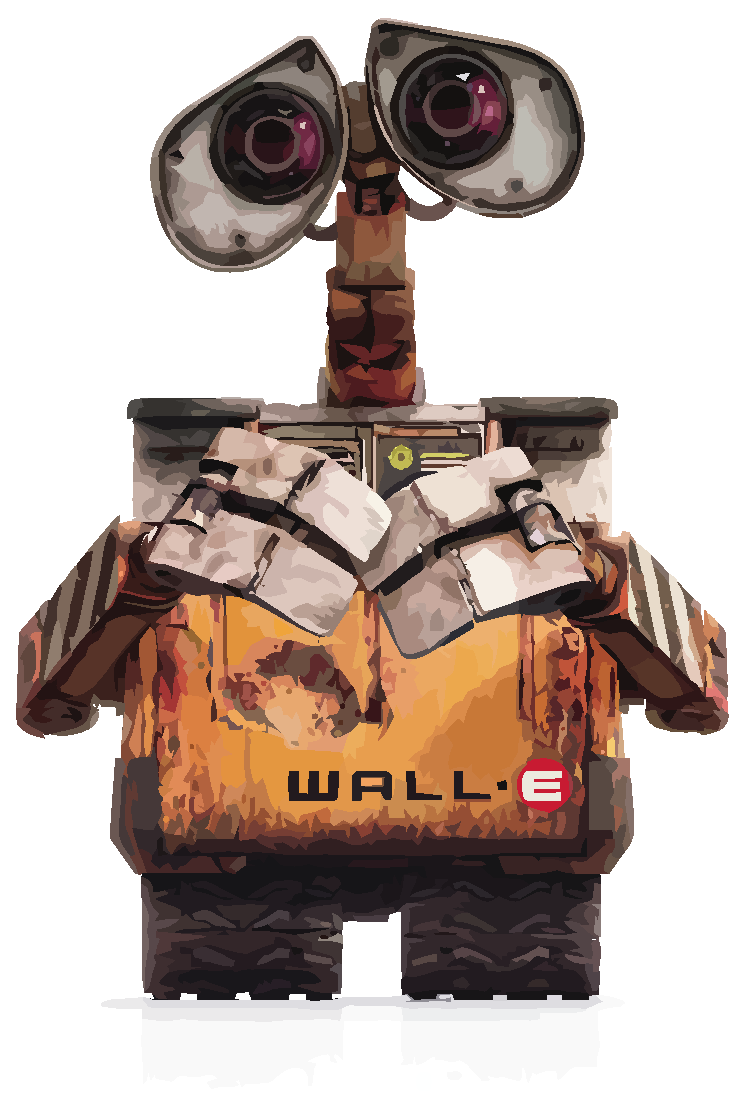
\includegraphics[width=\textwidth]{WallE}
    \caption{Wall-E}
    \label{fig:WallE}
  \end{subfigure}             
  \begin{subfigure}[b]{0.3\textwidth}
    
\includegraphics[width=\textwidth]{minion}
    \caption{Minions}
    \label{fig:Minnion}
  \end{subfigure}
  \caption{Best Animations}
  \label{fig:animations}
\end{figure}


\end{landscape}
